\documentclass[a4paper,14pt]{extreport}
\usepackage[russian]{babel}
\usepackage[left=3cm, right=1.5cm, top=2cm, bottom=2cm]{geometry}
\usepackage{amsmath}
\usepackage{titlesec}
\usepackage{graphicx}
\usepackage{float}%"Плавающие" картинки
\usepackage{wrapfig}%Обтекание фигур (таблиц, картинок и прочего)
\usepackage{longtable}
\usepackage{caption}

\titleformat{\section}{\filcenter\normalfont\large\bfseries}{\thesection.}{0.2em}{}
\titleformat{\subsection}{\filcenter\normalfont\large\bfseries}{\thesubsection.}{1em}{}
\renewcommand{\baselinestretch}{1.5}
\RequirePackage{caption}
\DeclareCaptionLabelSeparator{point}{ -- }
\captionsetup{justification=centering,labelsep=point}
\usepackage{tcolorbox}
\begin{document}
	\renewcommand\contentsname{Содержание}
	\renewcommand{\arraystretch}{1.3} 
	\thispagestyle{empty}
	\begin{center}
		Министерство науки и высшего образования Российской Федерации\\
        Федеральное государственное автономное образовательное\\
        учреждение высшего образования
		\vspace{0.1cm}
		
		«Казанский (Приволжский)  Федеральный университет
		\vspace{1cm}
		
		ИНСТИТУТ ВЫЧИСЛИТЕЛЬНОЙ МАТЕМАТИКИ И ИНФОРМАЦИОННЫХ ТЕХНОЛОГИЙ
		
		Кафедра прикладной математики и искусственного интеллекта

		\vspace{1cm}

		Направление подготовки: 01.03.04 - «Прикладная математика»
	\end{center}
	\vspace{1cm}
	
	\begin{center}
		КУРСОВАЯ РАБОТА
		\vspace{0.2cm}
		
		по дисциплине: «Численные методы»
		\vspace{0.2cm}
		
		\textbf{Система типа хищник-жертва. Модель Мак-Артура.}
	\end{center}
	\vspace{3cm}
	Студент 2 курса\\
	группы 09-222\\
	«\underline{\qquad}» \underline{\qquad\qquad} 2024 г. \qquad\qquad\quad \underline{\qquad\qquad\qquad\quad} \qquad Л.Ф. 	Фаррахова\\
	Научный руководитель\\
	ассистент б. с.\\
	«\underline{\qquad}» \underline{\qquad\qquad} 2024 г. \qquad\qquad\quad \underline{\qquad\qquad\qquad\quad} \qquad О.В. 	Глазырина
	\vspace{2cm}
	
	\begin{center}
		Казань, 2024
	\end{center}
	\newpage
	
	\setcounter{page}{2}
	\tableofcontents
	\newpage
	
	\begin{center}
		\section*{1 Постановка задачи}
		\addcontentsline{toc}{section}{1 Постановка задачи}
	\end{center}

    \par Рассмотрим динамику популяции двух видов, взаимодействующих между собой по типу хищник-жертва, при наличии внутривидовой конкуренции жертв за ограниченные ресурсы и при учете фактора насыщения хищника. Обозначим через $x=x(t)$ и $y=y(t)$ плотности популяций жертв и хищников в момент времени t. Уравнения имеют следующий вид:\par 

\begin{equation}
    \begin{aligned}
        \dfrac{d x}{d t} &= a\left(1-\dfrac{x}{K}\right)x - \dfrac{bxy}{1+Ax}, \\
        \dfrac{d y}{d t} &= -cy + \dfrac{d}{1+Ax}xy.
    \end{aligned}
\end{equation}


где $a$,$b$,$c$,$d$,$A$,$K$ - неотрицательные числа. Структура уравнений следующая:

\begin{itemize}
  \item 	Слагаемое $a\left(1-\dfrac{x}{K}\right)x$ определяет скорость размножения жертв в отсутствии хищников. При малых $x$ скорость определяется величиной $a$ и, таким образом, a характеризует норму рождаемости при малой плотности популяции. При большой плотности (до величины $K$) популяция растёт, при $x>K$ - уменьшается в размерах (скорость отрицательна). Таким образом, это слагаемое описывает ограниченность ресурсов: окружающая среда может обеспечивать существование только популяции плотности меньшей $K$.
  \item 	Слагаемое $\dfrac{bxy}{1+Ax}$ описывает влияние хищников на популяцию жертв. Функция $\dfrac{bx}{1+Ax}$ характеризует количество жертв, убиваемых одним хищником в единицу времени (реакция хищника на плотность популяции жертвы). Здесь учтено, что при большой плотности жертв хищник убивает лишь $\dfrac{b}{A}$ жертв в единицу времени; то есть перестаёт убивать когда насыщается.
  \item 	Второе уравнение определяет изменение популяции хищников. Постоянная c определяется естественной нормой смертности хищников. Второе слагаемое характеризует прирост хищников в зависимости от плотности жертв (функция $\dfrac{d}{1+Ax}$). При большой плотности жертв скорость прироста хищников определяется величиной $\dfrac{d}{A}$ и, таким образом, $\dfrac{d}{A}$ характеризует норму рождаемости при благоприятных для хищников условиях.
\end{itemize}


\subsubsection{Безразмерная форма уравнений} 
\hspace{0.8cm} Вводя безразмерные величины
$$
X=\left(\dfrac {d}{c}\right) x, \quad Y=\left(\dfrac{\mathrm{b}}{\mathrm{a}}\right) \mathrm{y}, \quad \tau=\mathrm{at}, \quad \alpha=\dfrac{\mathrm{Ac}}{\mathrm{d}}, \quad \epsilon=\dfrac{\mathrm{c}}{\mathrm{Kd}}, \quad \gamma=\dfrac{\mathrm{c}}{\mathrm{a}},
$$

преобразуем уравнения (1) к виду

\begin{equation}
    \begin{aligned}
        \dfrac{d X}{d \tau} &= (1-\epsilon X) X-\dfrac{X Y}{1+\alpha X}, \\
        \dfrac{d Y}{d \tau} &= \gamma \left(\dfrac{X}{1+\alpha X} - 1\right) Y, 
    \end{aligned}
\end{equation}

И дополним их начальньми условиями

\begin{equation}
\mathbf{X}(0)=\mathbf{X}_0, \mathbf{Y}(0)=\mathbf{Y}_0
\end{equation}

\subsubsection{Метод решения задачи Коши} 
\hspace{0.8cm}Для решения задачи (2) - (3) использовать метод Рунге-Кутты 4-го порядка точности (правило 3/8):


\begin{equation}
\begin{aligned}
k_1&=f\left(t_n, y_n\right), \\
k_2&=f\left(t_n+h / 3, y_n+h k_1 / 3\right), \\
k_3&=f\left(t_n+2 h / 3, y_n-h k_1 / 3+h k_2\right), \\
k_4&=f\left(t_n+h, y_n+h k_1-h k_2+h k_3\right), \\
y_{n+1}&=y_n+h\left(k_1+3 k_2+3 k_3+k_4\right) / 8;\\
\end{aligned}
\end{equation}

с постоянньм шагом $\mathrm{h}$. Для проверки правильности работы программы решить тестовую задачу из двух уравнений

\begin{equation}
    \begin{aligned}
y_1^{\prime}=y_1 /(2+2 t)-2 \mathrm{ty}_2, \quad y_2^{\prime}=y_2 /(2+2 t)+2 t y_1
    \end{aligned}
\end{equation}

на отрезке $[0,2]$ с точным решением\\
 \begin{equation*}
    \begin{aligned}
y_1=\cos \left(t^2\right) \sqrt{1+t}, \quad y_2=\sin \left(t^2\right) \sqrt{1+t}
    \end{aligned}
\end{equation*}

В ходе работы необходимо выполнить следующие действия:
	
	\begin{enumerate}
	 \item Проверить правильность вывода исходных уравнений (1), уравнений в безразмерном виде (2) и тестового решения (5).
	 \item Найти стационарные решения (состояния равновесия) системы (2)
	\item Написать процедуру интегрирования задачи Коши для системы из $\mathrm{n}$ обыкновенных дифференциальных уравнений по формулам (4) на произвольном отрезке $[a, b]$ c постоянным шагом $\mathrm{h}$.
  	\item Для тестовой задачи (5) построить графики зависимости максимальной погрешности решения е и $e / h^4$ от выбранного шага $h$.
  	\item Для значений параметра $\alpha$ из интервала $[0.1,0.9]$ рассчитать динамику популяции при следующих исходных данных

$$
\epsilon=0.1, \quad \gamma=1, \quad X_0=3, \quad Y_0=1
$$

Определите те значения параметра $\alpha$ при которых в системе появляются и исчезают устойчивые колебания (предельный цикл). Приведите графики наиболее характерных решений в координатах $(X, Y), \newline(\mathrm{X}(\mathrm{t}),  \mathrm{t})$ и $(\mathrm{Y}(\mathrm{t}), \mathrm{t})$ и дайте их интергретацию.
	\end{enumerate}


	\newpage
	
	\section*{3 Ход работы}
	\addcontentsline{toc}{section}{3 Ход работы}

    \par \hspace{0.8cm}Для перехода от системы уравнений (1) к системе уравнений (2) введем новые переменные и новые параметры, а затем проведем соответствующие замены и преобразования.

    Введем следующие замены:
    \begin{align*}
    X &= \dfrac{d}{c} x, \\
    Y &= \dfrac{b}{a} y, \\
    \tau &= at,
    \end{align*}
    где $\tau$ - новая безразмерная переменная времени.
    
    Также введем новые параметры:
    \begin{align*}
    \alpha &= \dfrac{Ac}{d}, \\
    \epsilon &= \dfrac{c}{Kd}, \\
    \gamma &= \dfrac{c}{a}.
    \end{align*}
    
    Найдем производные:
    \begin{equation*}
    \dfrac{dx}{dt} = \dfrac{d \left( \dfrac{c}{d} X \right)}{d \left( \dfrac{\tau}{a} \right)} = \dfrac{c}{d} \cdot a \dfrac{dX}{d\tau}, \quad \dfrac{dy}{dt} = \dfrac{d \left( \dfrac{a}{b} Y \right)}{d \left( \dfrac{\tau}{a} \right)} = \dfrac{a}{b} \cdot a \dfrac{dY}{d\tau}.
    \end{equation*}
    
    Подставим новые переменные и производные в исходные уравнения:
    \begin{equation*}
    \dfrac{c}{d} \cdot a \dfrac{dX}{d\tau} = a\left(1 - \dfrac{\dfrac{c}{d} X}{K}\right) \dfrac{c}{d} X - \dfrac{b \dfrac{c}{d} X \dfrac{a}{b} Y}{1 + A \dfrac{c}{d} X},
    \end{equation*}
    \begin{equation*}
    \dfrac{a}{b} \cdot a \dfrac{dY}{d\tau} = -c \cdot \dfrac{a}{b} Y + \dfrac{d \cdot \dfrac{a}{b} Y \cdot \dfrac{c}{d} X}{1 + A \dfrac{c}{d} X}.
    \end{equation*}
    \newpage
    Сократим на соответствующие коэффициенты:
    \begin{equation*}
    \dfrac{ca}{d} \dfrac{dX}{d\tau} = a \left(1 - \dfrac{cX}{Kd}\right) \dfrac{cX}{d} - \dfrac{cXY}{d(1 + \dfrac{AcX}{d})},
    \end{equation*}
    \begin{equation*}
    a \dfrac{dY}{d\tau} = -c \dfrac{aY}{b} + \dfrac{aXY}{b(1 + \dfrac{AcX}{d})}.
    \end{equation*}
    
    Применив параметры $\epsilon = \dfrac{c}{Kd}$, $\alpha = \dfrac{Ac}{d}$ и $\gamma = \dfrac{c}{a}$, получим систему уравнений (2):
    \begin{equation*}
    \dfrac{dX}{d\tau} = (1 - \epsilon X) X - \dfrac{XY}{1 + \alpha X},
    \end{equation*}
    \begin{equation*}
    \dfrac{dY}{d\tau} = \gamma \left(\dfrac{X}{1 + \alpha X} - 1\right) Y.
    \end{equation*}
    дополненную начальными условиями:
    \begin{equation*}
    X(0) = X_0, \quad Y(0) = Y_0.
    \end{equation*}

\par Для того, чтобы проверить правильность работы метода Рунге-Кутты, решим тестовую задачу (5).

Для доказательства, что $y_1(t) = \cos(t^2) \sqrt{1+t}$ и $y_2(t) = \sin(t^2) \sqrt{1+t}$ являются решениями данной системы дифференциальных уравнений, мы должны подставить их в уравнения и проверить, что они удовлетворяют исходной системе.

Подставим $y_1(t) = \cos(t^2) \sqrt{1+t}$ и $y_2(t) = \sin(t^2) \sqrt{1+t}$ в первое уравнение:
\begin{align*}
y_1' &= \dfrac{y_1}{2+2t} - 2ty_2 = \dfrac{\cos(t^2) \sqrt{1+t}}{2+2t} - 2t \sin(t^2) \sqrt{1+t}.
\end{align*}

Подставим $y_1(t) = \cos(t^2) \sqrt{1+t}$ и $y_2(t) = \sin(t^2) \sqrt{1+t}$ во второе уравнение:
\begin{align*}
y_2' &= \dfrac{y_2}{2+2t} + 2ty_1 = \dfrac{\sin(t^2) \sqrt{1+t}}{2+2t} + 2t \cos(t^2) \sqrt{1+t}.
\end{align*}

Теперь проверим, удовлетворяют ли эти выражения исходной системе уравнений:

\begin{align*}
\dfrac{\cos(t^2) \sqrt{1+t}}{2+2t} - 2t \sin(t^2) \sqrt{1+t} &= \dfrac{y_1}{2+2t} - 2ty_2 = y_1', \\
\dfrac{\sin(t^2) \sqrt{1+t}}{2+2t} + 2t \cos(t^2) \sqrt{1+t} &= \dfrac{y_2}{2+2t} + 2ty_1 = y_2'.
\end{align*}

Таким образом, подставив $y_1(t) = \cos(t^2) \sqrt{1+t}$ и $y_2(t) = \sin(t^2) \sqrt{1+t}$ в исходную систему дифференциальных уравнений, мы видим, что они являются решениями этой системы.

Построим график полученных решений методом Рунге-Кутты и график точного решения для погрешностей для $x(t)$ и $y(t)$, выбрав количество разбиений равным 100.

\begin{center}
\begin{minipage}[htb]{0.8\linewidth}
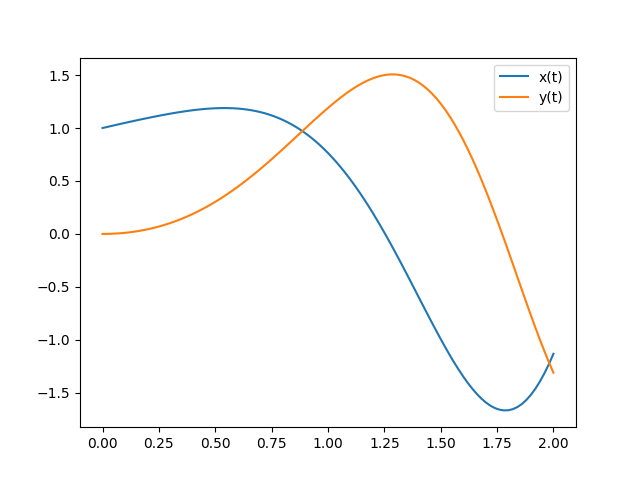
\includegraphics[width=14cm]{1.png}
\end{minipage}
\end{center}
\begin{center}
Рисунок 1 - График полученного решения методом Рунге-Кутты
\end{center}
\begin{center}
\begin{minipage}[htb]{0.8\linewidth}
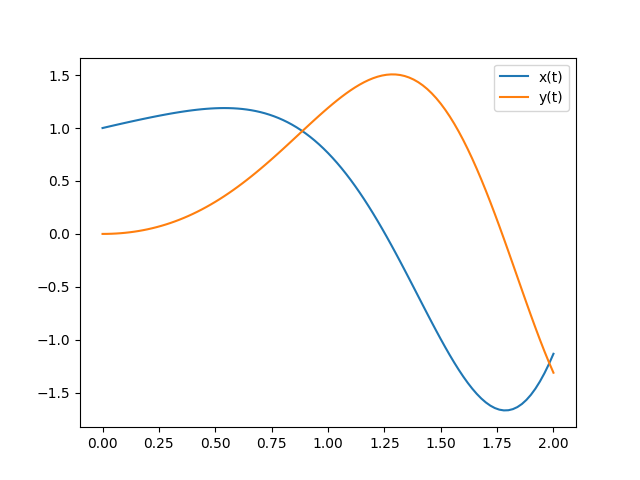
\includegraphics[width=14cm]{2.png}
\end{minipage}
\end{center}
\begin{center}
Рисунок 2 -  График точного решения
\end{center}

Сравнивая рисунки 1-2 визуально определить погрешность достаточно сложно, поэтому вычислим максимальную погрешность $e$ и $e/h^4$ в зависи\-мости от $n$ и построим график, где по оси ординат - максимальная ошибка, а по оси абсцисс количество разбиений($n$):
\begin{center}
    \begin{minipage}[htb]{0.7\linewidth}
    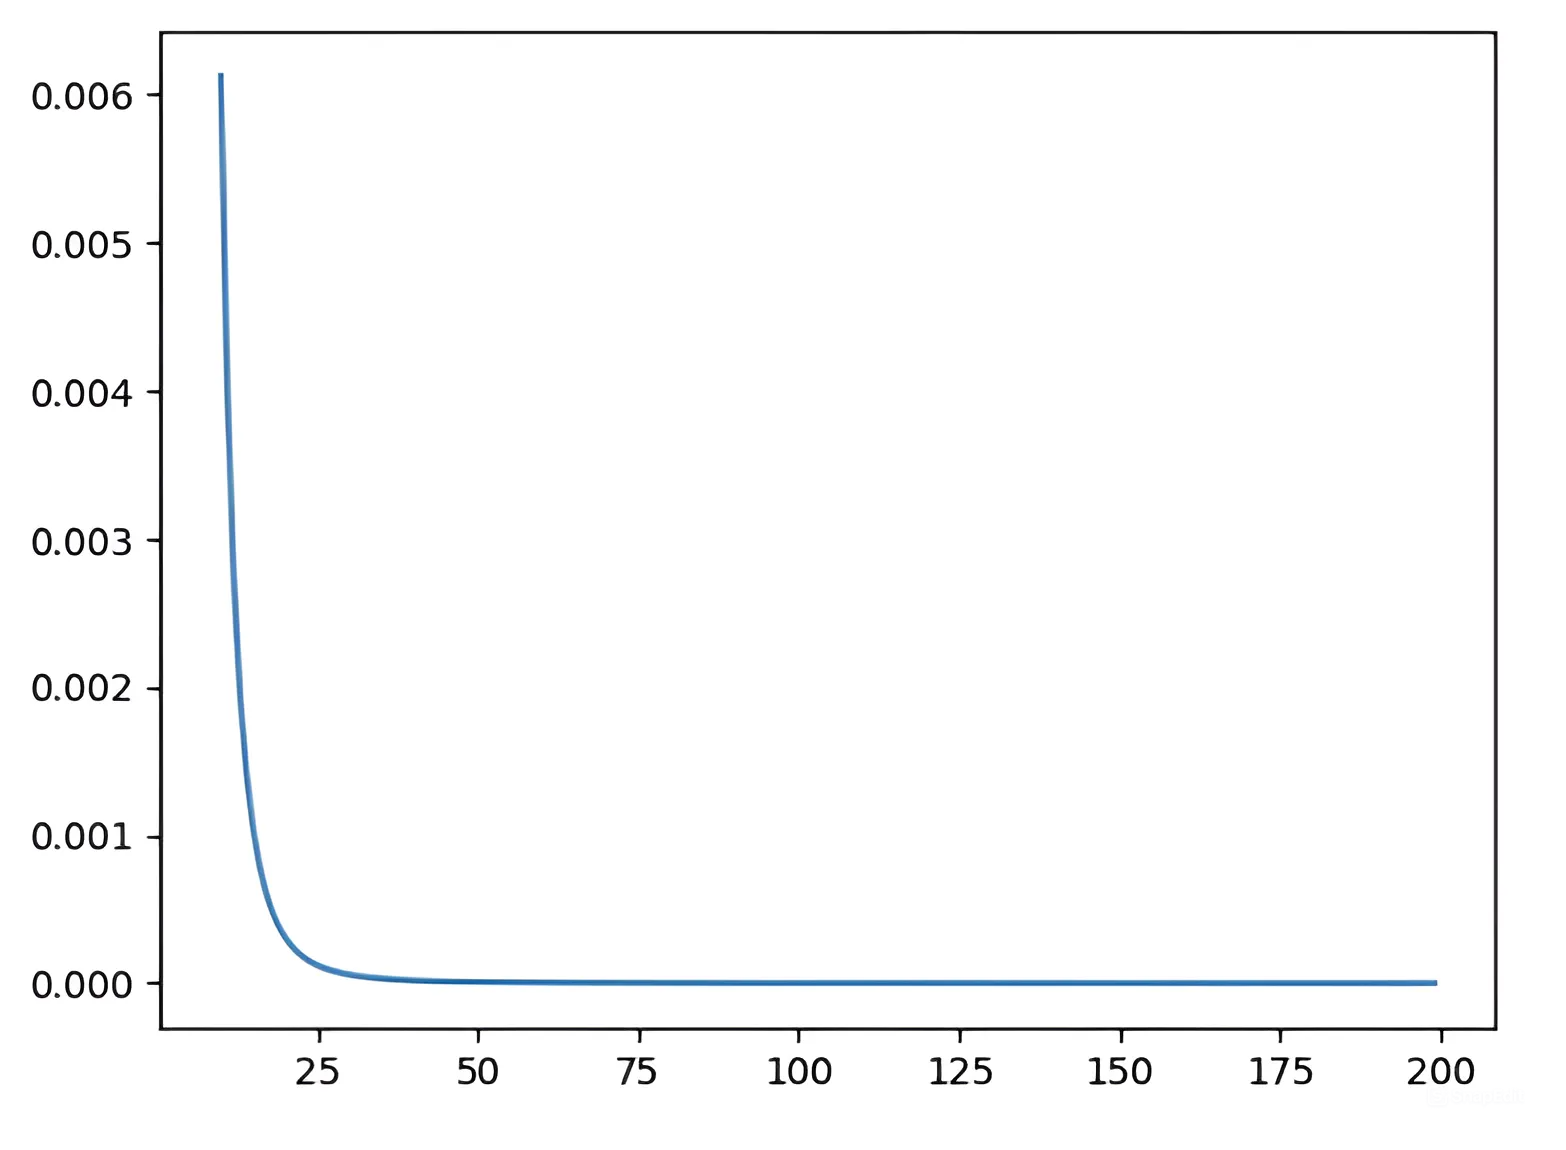
\includegraphics[width=12cm]{3.png}
    \end{minipage}
    \end{center}
    \begin{center}
    Рисунок 3 - График зависимости погрешности от шага h.
    \end{center}
    \begin{center}
    \begin{minipage}[htb]{0.7\linewidth}
    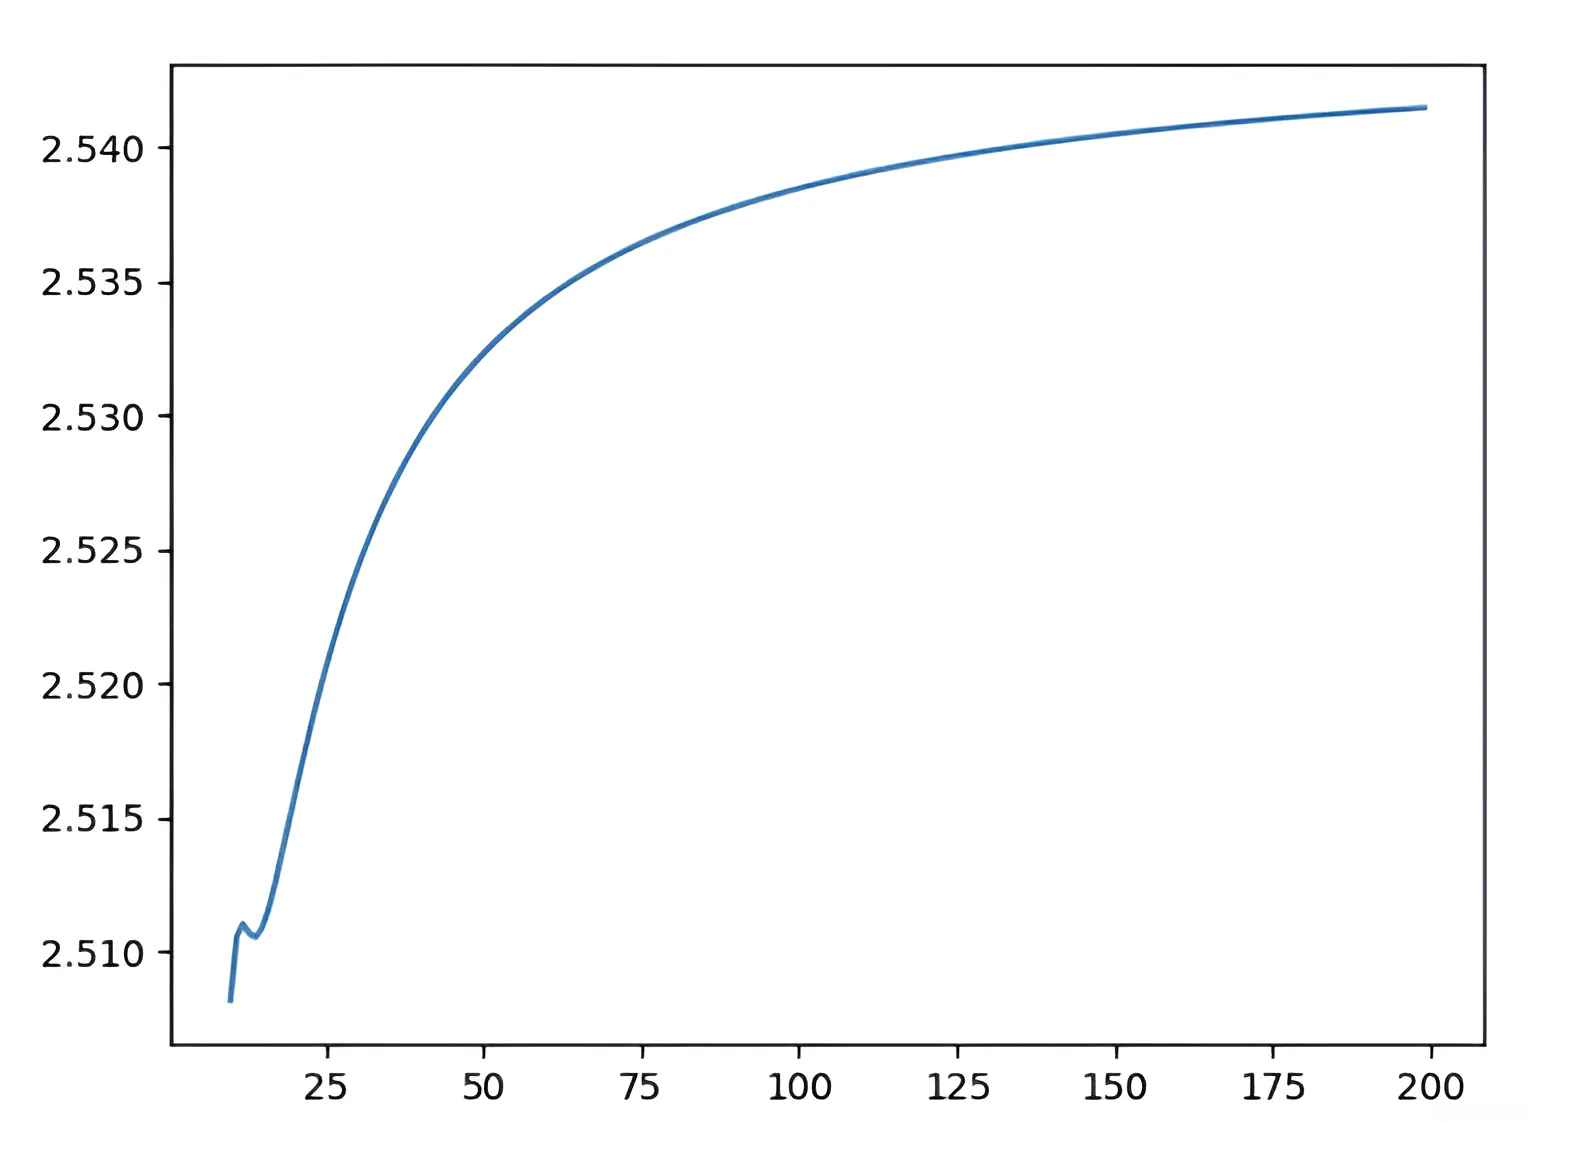
\includegraphics[width=12cm]{4.png}
    \end{minipage}
    \end{center}
    \begin{center}
    Рисунок 4 - График зависимости погрешности от шага $h^4$.
    \end{center}


По графикам можно сделать вывод, что максимальная погрешность решения e возрастает при увеличении шага h.

Далее найдем стационарные решения системы (2). Для этого приравняем производняе к нулю и решим полученные уравнения. Итак, для данной системы уравнений стационарные решения будут удовлетворять следующим уравнениям:

\begin{equation*}
    \begin{aligned}
        (1-\epsilon X) X-\dfrac{X Y}{1+\alpha X} = 0, \\
        \gamma \left(\dfrac{X}{1+\alpha X} - 1\right) Y = 0, 
    \end{aligned}
\end{equation*}

Первое уравнение можно переписать в виде:

\begin{equation*}
    \begin{aligned}
        X \left(1 - \epsilon X - \dfrac{Y}{1+\alpha X}\right) = 0
    \end{aligned}
\end{equation*}

Отсюда следует, что

\begin{equation*}
    \begin{aligned}
        X = 0 \text{ или } 1-\epsilon X -\dfrac{Y}{1+\alpha X} = 0
    \end{aligned}
\end{equation*}

Второе уравнение можно переписать в виде:

\begin{equation*}
    \begin{aligned}
       Y \left(\gamma \left(\dfrac{X}{1+\alpha X} \right) \right) = 0
    \end{aligned}
\end{equation*}

Отсюда следует, что

\begin{equation*}
    \begin{aligned}
       Y = 0 \text{ или } \gamma \left(\dfrac{X}{1+\alpha X} - 1 \right) = 0
    \end{aligned}
\end{equation*}

Таким образом, решив эту систему уравнений, мы найдем состояния равновесия системы дифференциальных уравнений, которые имеют вид:

\begin{equation*}
    \begin{aligned}
       (X,Y)=(0,0) \text{ или } (X,Y)=(-\dfrac{1}{\alpha},\gamma \dfrac{1-\alpha}{\alpha})
    \end{aligned}
\end{equation*}

Далее для значений параметра $\alpha$ из интервала $[0.1, 0.9]$ рассчитаем динамику популяции при следующих исходных данных

$$
\epsilon=0.1, \quad \gamma=1, \quad X_0=3, \quad Y_0=1
$$

Приведем графики в координатах $(X,Y), (X(t),t)$ и $(Y(t),t)$


\begin{center}
    \begin{minipage}[htb]{0.8\linewidth}
    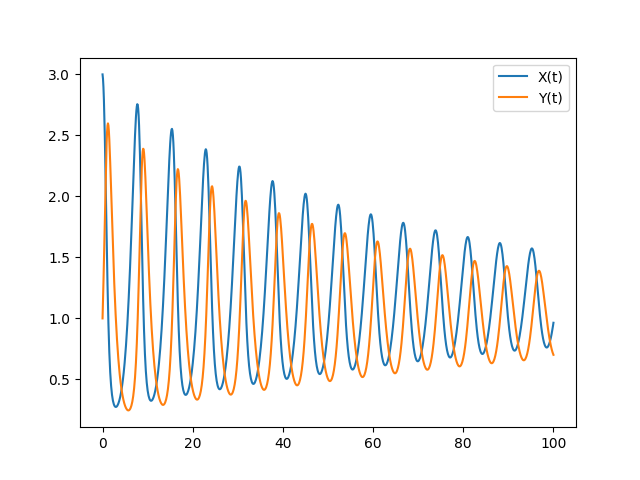
\includegraphics[width=14cm]{n5.png}
    \end{minipage}
    \end{center}
    \begin{center}
        Рисунок 5 - График динамики популяции при $\alpha = 0.1$ в координатах $(X(t),t),(Y(t),t)$
    \end{center}
    \begin{center}
    \begin{minipage}[htb]{0.8\linewidth}
    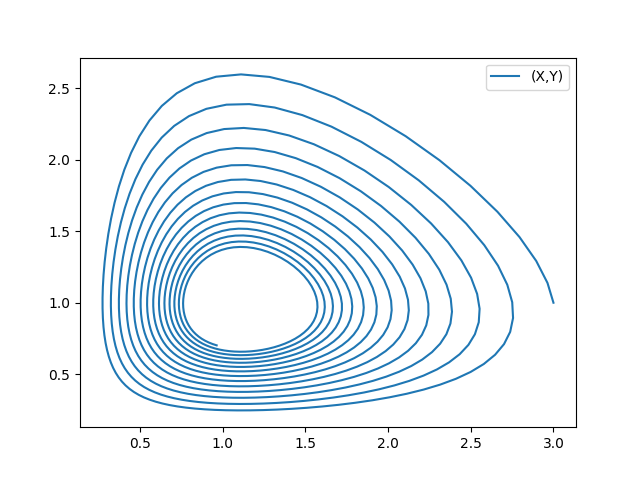
\includegraphics[width=14cm]{5.png}
    \end{minipage}
    \end{center}
    \begin{center}
        Рисунок 6 - График динамики популяции при $\alpha = 0.1$ в координатах $(X,Y)$  
    \end{center}

\begin{center}
    \begin{minipage}[htb]{0.8\linewidth}
    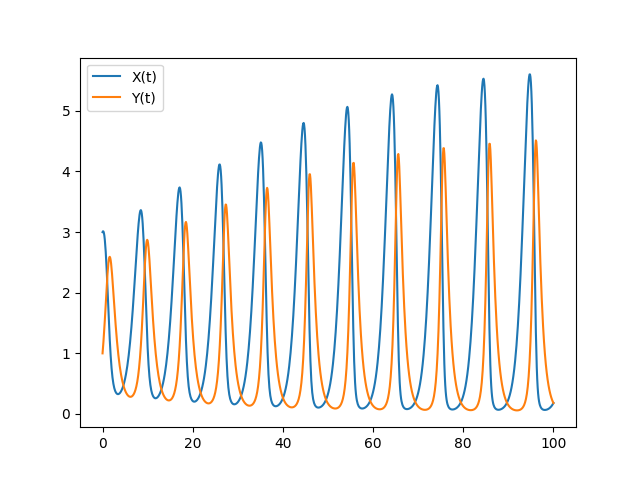
\includegraphics[width=14cm]{n6.png}
    \end{minipage}
    \end{center}
    \begin{center}
        Рисунок 7 - График динамики популяции при $\alpha = 0.2$ в координатах $(X(t),t),(Y(t),t)$
    \end{center}
    \begin{center}
    \begin{minipage}[htb]{0.8\linewidth}
    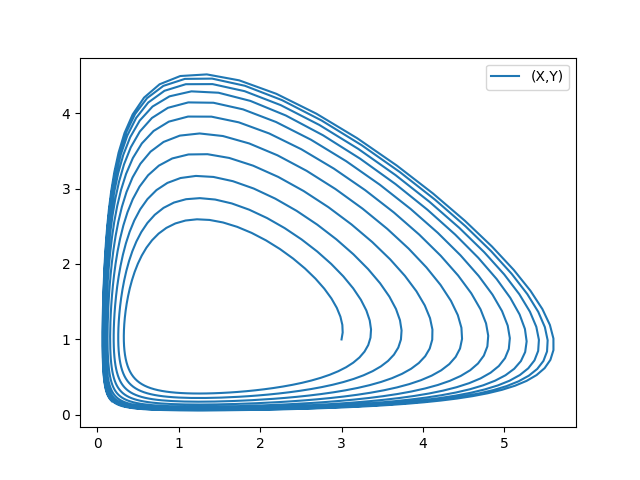
\includegraphics[width=14cm]{6.png}
    \end{minipage}
    \end{center}
    \begin{center}
        Рисунок 8 - График динамики популяции при $\alpha = 0.2$ в координатах $(X,Y)$  
    \end{center}

\begin{center}
    \begin{minipage}[htb]{0.8\linewidth}
    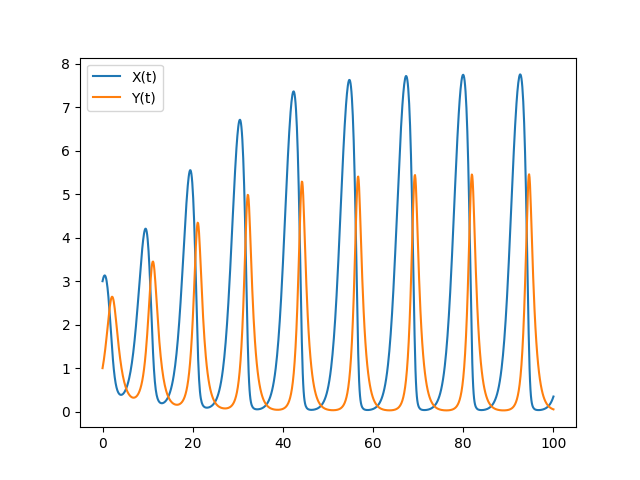
\includegraphics[width=14cm]{n7.png}
    \end{minipage}
    \end{center}
    \begin{center}
        Рисунок 9 - График динамики популяции при $\alpha = 0.3$ в координатах $(X(t),t),(Y(t),t)$
    \end{center}
    \begin{center}
    \begin{minipage}[htb]{0.8\linewidth}
    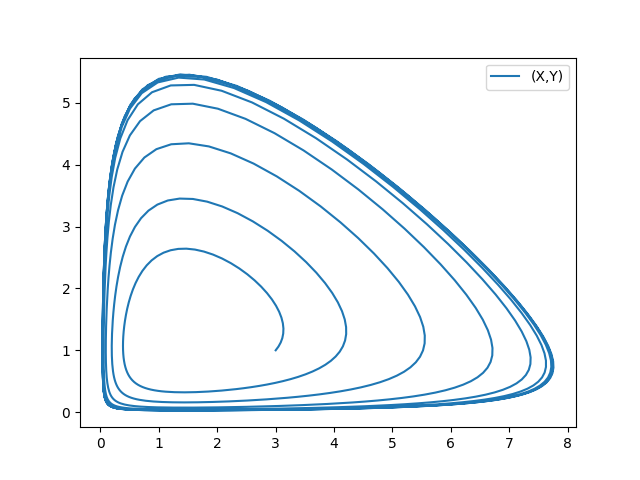
\includegraphics[width=14cm]{7.png}
    \end{minipage}
    \end{center}
    \begin{center}
        Рисунок 10 - График динамики популяции при $\alpha = 0.3$ в координатах $(X,Y)$  
    \end{center}

\begin{center}
    \begin{minipage}[htb]{0.8\linewidth}
    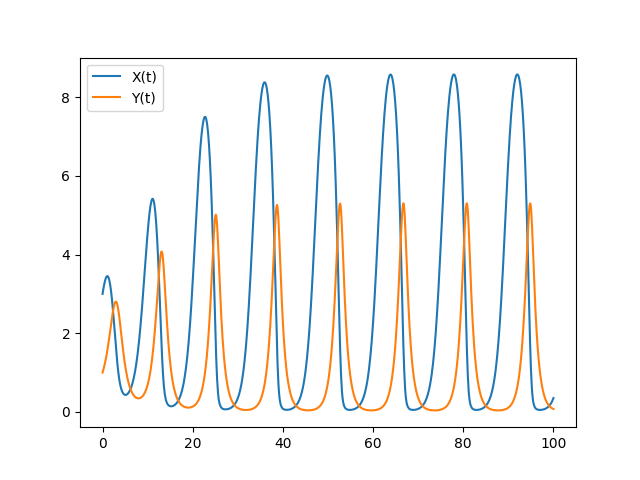
\includegraphics[width=14cm]{n8.png}
    \end{minipage}
    \end{center}
    \begin{center}
        Рисунок 11 - График динамики популяции при $\alpha = 0.4$ в координатах $(X(t),t),(Y(t),t)$
    \end{center}
    \begin{center}
    \begin{minipage}[htb]{0.8\linewidth}
    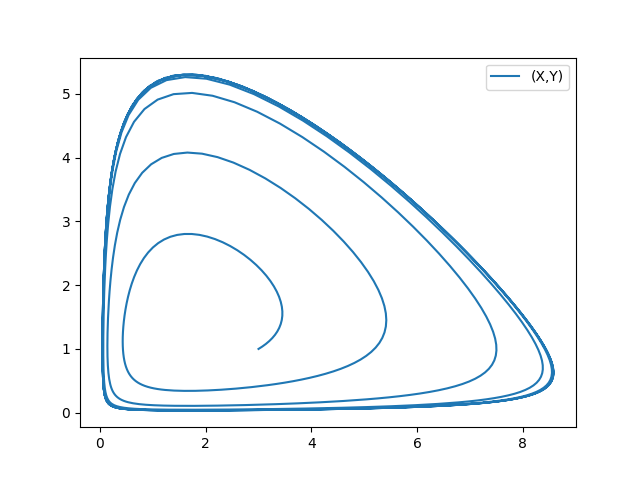
\includegraphics[width=14cm]{8.png}
    \end{minipage}
    \end{center}
    \begin{center}
        Рисунок 12 - График динамики популяции при $\alpha = 0.4$ в координатах $(X,Y)$  
    \end{center}

\begin{center}
    \begin{minipage}[htb]{0.8\linewidth}
    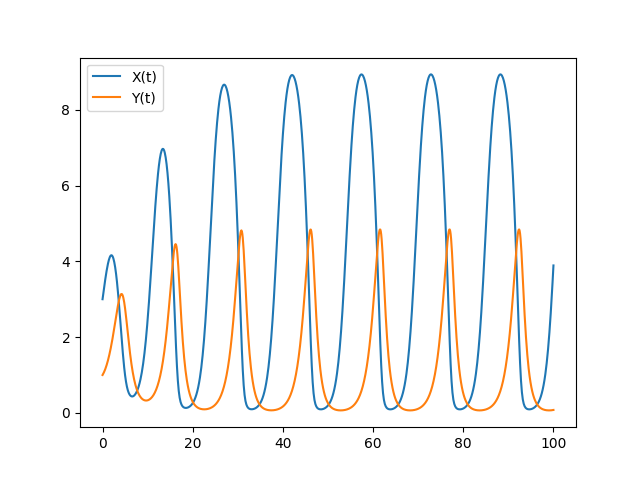
\includegraphics[width=14cm]{n9.png}
    \end{minipage}
    \end{center}
    \begin{center}
        Рисунок 13 - График динамики популяции при $\alpha = 0.5$ в координатах $(X(t),t),(Y(t),t)$
    \end{center}
    \begin{center}
    \begin{minipage}[htb]{0.8\linewidth}
    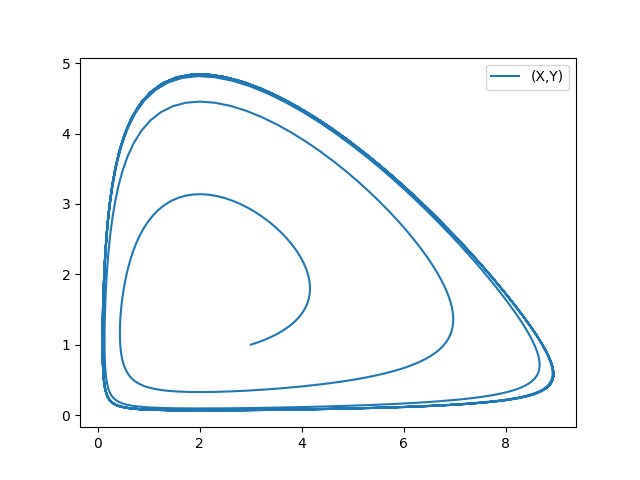
\includegraphics[width=14cm]{9.png}
    \end{minipage}
    \end{center}
    \begin{center}
        Рисунок 14 - График динамики популяции при $\alpha = 0.5$ в координатах $(X,Y)$  
    \end{center}

\begin{center}
    \begin{minipage}[htb]{0.8\linewidth}
    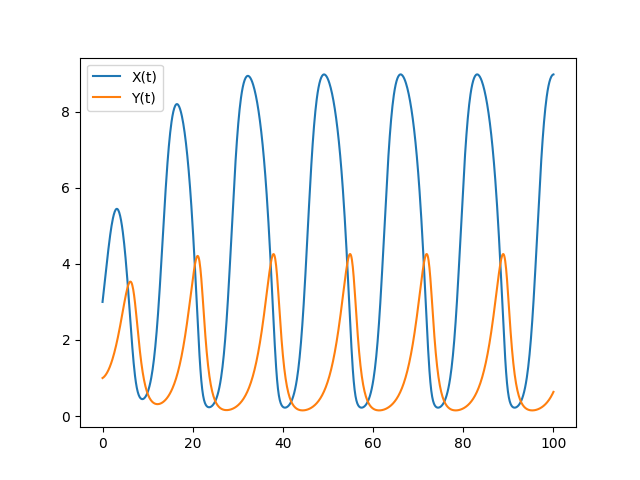
\includegraphics[width=14cm]{n10.png}
    \end{minipage}
    \end{center}
    \begin{center}
        Рисунок 15 - График динамики популяции при $\alpha = 0.6$ в координатах $(X(t),t),(Y(t),t)$
    \end{center}
    \begin{center}
    \begin{minipage}[htb]{0.8\linewidth}
    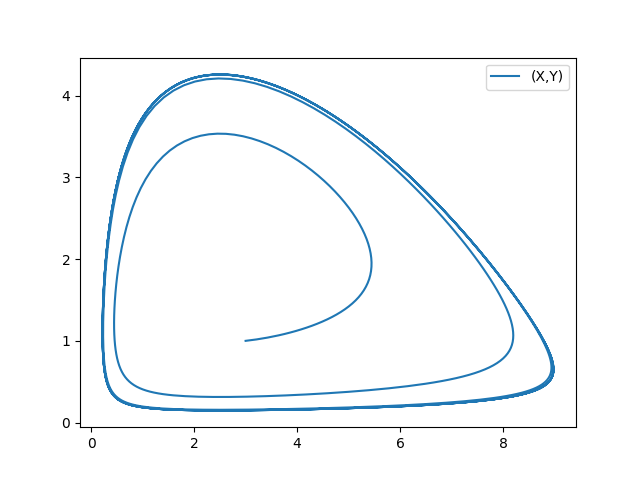
\includegraphics[width=14cm]{10.png}
    \end{minipage}
    \end{center}
    \begin{center}
        Рисунок 16 - График динамики популяции при $\alpha = 0.6$ в координатах $(X,Y)$  
    \end{center}

\begin{center}
    \begin{minipage}[htb]{0.8\linewidth}
    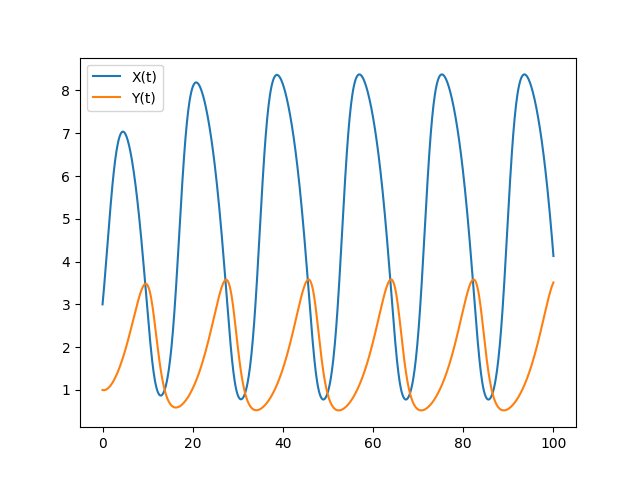
\includegraphics[width=14cm]{n11.png}
    \end{minipage}
    \end{center}
    \begin{center}
        Рисунок 17 - График динамики популяции при $\alpha = 0.7$ в координатах $(X(t),t),(Y(t),t)$
    \end{center}
    \begin{center}
    \begin{minipage}[htb]{0.8\linewidth}
    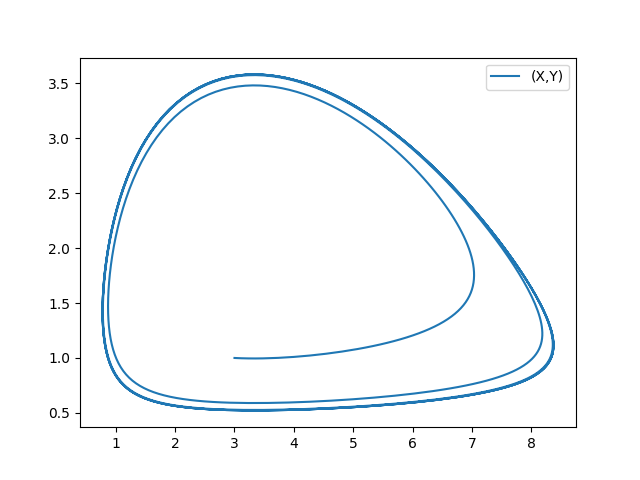
\includegraphics[width=14cm]{11.png}
    \end{minipage}
    \end{center}
    \begin{center}
        Рисунок 18 - График динамики популяции при $\alpha = 0.7$ в координатах $(X,Y)$  
    \end{center}

\begin{center}
    \begin{minipage}[htb]{0.8\linewidth}
    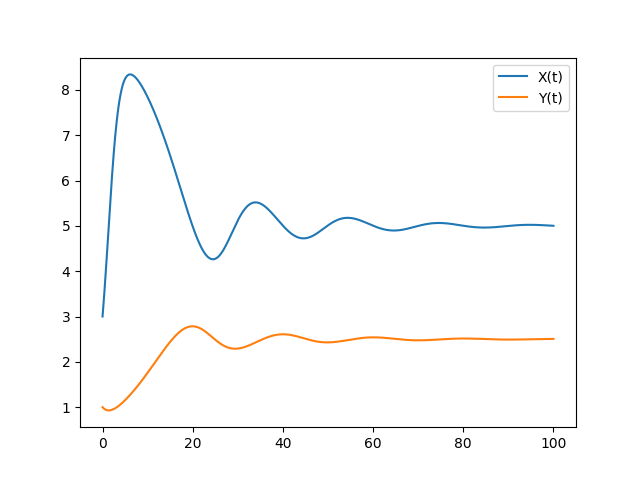
\includegraphics[width=14cm]{n12.png}
    \end{minipage}
    \end{center}
    \begin{center}
        Рисунок 19 - График динамики популяции при $\alpha = 0.8$ в координатах $(X(t),t),(Y(t),t)$
    \end{center}
    \begin{center}
    \begin{minipage}[htb]{0.8\linewidth}
    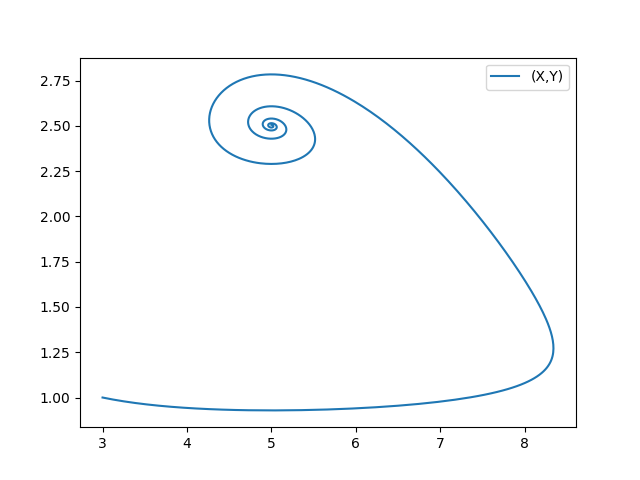
\includegraphics[width=14cm]{12.png}
    \end{minipage}
    \end{center}
    \begin{center}
        Рисунок 20 - График динамики популяции при $\alpha = 0.8$ в координатах $(X,Y)$  
    \end{center}

\begin{center}
    \begin{minipage}[htb]{0.8\linewidth}
    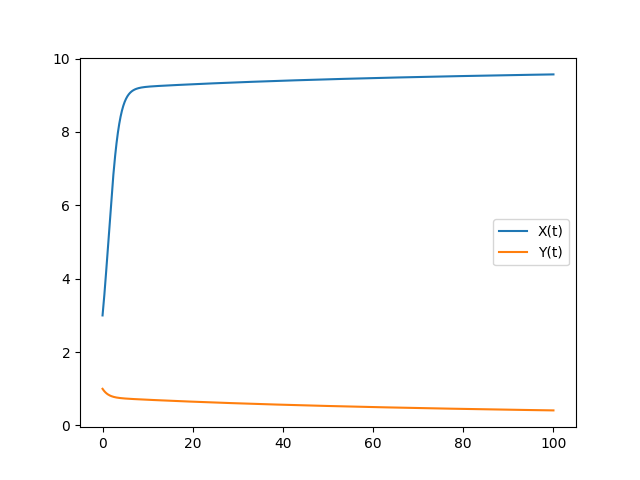
\includegraphics[width=14cm]{n13.png}
    \end{minipage}
    \end{center}
    \begin{center}
        Рисунок 21 - График динамики популяции при $\alpha = 0.9$ в координатах $(X(t),t),(Y(t),t)$
    \end{center}
    \begin{center}
    \begin{minipage}[htb]{0.8\linewidth}
    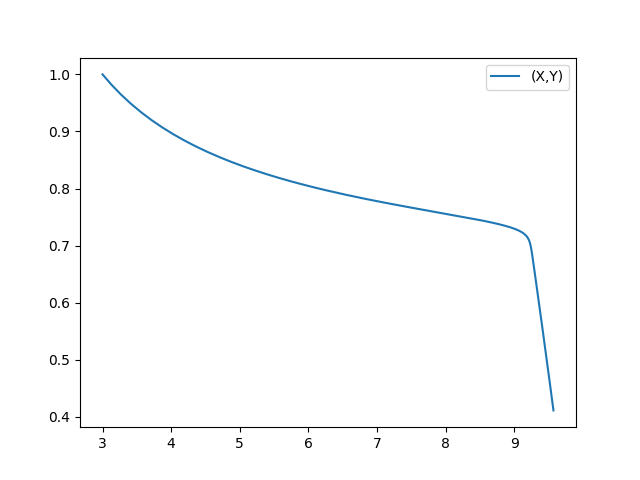
\includegraphics[width=14cm]{13.png}
    \end{minipage}
    \end{center}
    \begin{center}
        Рисунок 22 - График динамики популяции при $\alpha = 0.9$ в координатах $(X,Y)$  
    \end{center}

    
На графиках в координатах (X, Y) мы можем увидеть, как изменяются значения переменных X и Y в зависимости от параметра $\alpha$.


При $\alpha$ = 0.1 и $\alpha$ = 0.8 система имеет устойчивый фокус, что означает, что популяции хищников и жертв со временем достигают равновесия. В этом случае популяции колеблются вокруг точки равновесия и в конечном итоге стабилизируются, не продолжая изменяться со временем.

Устойчивые фокусы указывают на то, что при определенных условиях экосистема может прийти в состояние стабильности, где популяции остаются постоянными.

При $\alpha \in (0.1, 0.7)$ система имеет неустойчивый фокус, что приводит к колебаниям популяций с увеличивающейся амплитудой до тех пор, пока они не достигнут предельного цикла. Предельный цикл представляет собой состояние, при котором популяции колеблются периодически и стабильно без затухания или роста амплитуды.

Неустойчивые фокусы и предельные циклы указывают на динамичную экосистему, где популяции хищников и жертв регулярно меняются, но эти изменения ограничены и предсказуемы.

Так, $\alpha$ влияет на насыщение хищников, т.е. на то, как быстро хищники достигают своего предельного уровня добычи при увеличении плотности популяции жертв.

Низкие значения $\alpha$ (например, 0.1) могут соответствовать ситуации, когда хищники быстро насыщаются и перестают увеличивать уровень добычи, что способствует установлению равновесия.
Средние значения $\alpha$ (например, 0.5) приводят к неустойчивым колебаниям и предельным циклам, что указывает на более сложные динамические взаимодействия между хищниками и жертвами.
Высокие значения $\alpha$ (например, 0.8) могут указывать на ситуацию, когда хищники медленно достигают насыщения, что также приводит к устойчивому равновесию.

Таким образом, учет насыщения хищников играет ключевую роль в динамике популяций. Он определяет, как хищники реагируют на изменения в популяции жертв и влияет на устойчивость системы. Внутривидовая конкуренция среди жертв также важна для достижения равновесия и предотвращения неконтролируемого роста популяций. 

Понимание того, при каких значениях параметров система переходит от устойчивого равновесия к колебаниям, важно для управления экосистемой. Это позволяет предсказать и, возможно, контролировать динамику популяций в реальных условиях.

\newpage
\section*{4 Вывод}
	\addcontentsline{toc}{section}{4 Вывод}
\par \hspace{0.8cm} В ходе выполнении курсовой работы, была решена тестовая задача и реализована программа интегрирования задачи Коши с 
помощью Рунге- Кутты 4-го порядка точности с постоянным шагом h. Были построены графики зависимости максимальной 
погрешности решения $e$ и $e/h^4$ от выбранного шага h. По графикам можно сделать вывод, что максимальная погрешность
решения e возрастает при увеличении шага h. Была построена модель Мак – Артура системы типа хищник-жертва. 

\newpage
\section*{5 Список литературы}
	\addcontentsline{toc}{section}{5 Список литературы}
\begin{enumerate}
  \item Даутов Р. З. Практикум по дисциплине “Численные методы”. Решение задачи Коши для системы ОДУ. - Учебное пособие, Казань, 2014.
  \item Эрроусмит Д., Плейс К. Обыкновенные дифференциальные уравнения. Качественная теория с приложениями. - М.: Мир, 1986.
  \item Хайрер Э., Нерсетт С., Ваннер Г. Решение обыкновенных дифференциальных уравнений. - М.: Мир, 1990.
  \item Самарский А.А., Гулин А.В. Численные методы. - М.: Наука, 1989.
  \item Бахвалов Н.С., Жидков Н.П., Кобельков Г.М. Численные методы. - М.: Наука, 1987.
\end{enumerate}


\newpage
\section*{6 Листинг}
	\addcontentsline{toc}{section}{6 Листинг}
Программа реализована на Python.\\
\begin{verbatim}
import numpy as np
import matplotlib.pyplot as plt

def fx_test(t, x, y):
    return x / (2 + 2 * t) - 2 * t * y

def fy_test(t, x, y):
    return y / (2 + 2 * t) + 2 * t * x

def fx_dynamic(t, x, y, alfa):
    eps = 0.1
    return (1 - eps * x) * x - (x * y) / (1 + alfa * x)

def fy_dynamic(t, x, y, alfa):
    gamma = 1
    return gamma * (x / (1 + alfa * x) - 1) * y

def solve_test(t1, t2, h, x0, y0):
    n = int((t2 - t1) / h + 1)
    t = np.linspace(t1, t2, n)
    x = np.zeros(n)
    y = np.zeros(n)
    x[0] = x0
    y[0] = y0

    for i in range(n - 1):
        xk1 = fx_test(t[i], x[i], y[i])
        yk1 = fy_test(t[i], x[i], y[i])
        xk2 = fx_test(t[i] + h / 3, x[i] + h * xk1/3, 
        y[i] + h * yk1 / 3)
        yk2 = fy_test(t[i] + h / 3, x[i] + h * xk1/3, 
        y[i] + h * yk1 / 3)
        xk3 = fx_test(t[i] + 2 * h / 3, x[i] - h * xk1/3 
        + h * xk2, y[i] - h * yk1 / 3 + h * yk2)
        yk3 = fy_test(t[i] + 2 * h / 3, x[i] - h * xk1/3 
        + h * xk2, y[i] - h * yk1 / 3 + h * yk2)
        xk4 = fx_test(t[i] + h, x[i] + h * (xk1 - xk2 + xk3), 
        y[i] + h * (yk1 - yk2 + yk3))
        yk4 = fy_test(t[i] + h, x[i] + h * (xk1 - xk2 + xk3), 
        y[i] + h * (yk1 - yk2 + yk3))
        x[i + 1] = x[i] + h * (xk1 + 3 * xk2 + 3 * xk3 + xk4)/8
        y[i + 1] = y[i] + h * (yk1 + 3 * yk2 + 3 * yk3 + yk4)/8

    return t, x, y

def solve_dynamic(t1, t2, h, x0, y0, alfa):
    n = int((t2 - t1) / h + 1)
    t = np.linspace(t1, t2, n)
    x = np.zeros(n)
    y = np.zeros(n)
    x[0] = x0
    y[0] = y0

    for i in range(n - 1):
        xk1 = fx_dynamic(t[i], x[i], y[i], alfa)
        yk1 = fy_dynamic(t[i], x[i], y[i], alfa)
        xk2 = fx_dynamic(t[i] + h / 3, x[i] + h * xk1/3, 
        y[i] + h * yk1 / 3, alfa)
        yk2 = fy_dynamic(t[i] + h / 3, x[i] + h * xk1/3, 
        y[i] + h * yk1 / 3, alfa)
        xk3 = fx_dynamic(t[i] + 2 * h / 3, x[i] - h * xk1/3 
        + h * xk2, y[i] - h * yk1 / 3 + h * yk2, alfa)
        yk3 = fy_dynamic(t[i] + 2 * h / 3, x[i] - h * xk1/3 
        + h * xk2, y[i] - h * yk1 / 3 + h * yk2, alfa)
        xk4 = fx_dynamic(t[i] + h, x[i] + h * (xk1 - xk2 
        + xk3), y[i] + h * (yk1 - yk2 + yk3), alfa)
        yk4 = fy_dynamic(t[i] + h, x[i] + h * (xk1 - xk2 
        + xk3), y[i] + h * (yk1 - yk2 + yk3), alfa)
        x[i + 1] = x[i] + h * (xk1 + 3 * xk2 + 3 * xk3 + xk4)/8
        y[i + 1] = y[i] + h * (yk1 + 3 * yk2 + 3 * yk3 + yk4)/8

    return t, x, y

def exact(t1, t2, h):
    n = int((t2 - t1) / h + 1)
    t = np.linspace(t1, t2, n)
    x = np.zeros(n)
    y = np.zeros(n)
    for i in range(n):
        x[i] = np.cos(t[i]**2) * np.sqrt(1 + t[i])
        y[i] = np.sin(t[i]**2) * np.sqrt(1 + t[i])
    return x, y

def main_test():
    t1 = 0
    t2 = 2
    x0 = 1
    y0 = 0
    n = 36

    # Решение методом Рунге-Кутты 4-го порядка
    N = 100
    h = (t2 - t1) / N
    t, x, y = solve_test(t1, t2, h, x0, y0)

    plt.figure()
    plt.plot(t, x, label='x(t)')
    plt.plot(t, y, label='y(t)')
    plt.legend()
    plt.savefig('1.png')
    plt.show()

    # Точное решение
    x1, y1 = exact(t1, t2, h)
    plt.figure()
    plt.plot(t, x1, label='xExact(t)')
    plt.plot(t, y1, label='yExact(t)')
    plt.legend()
    plt.savefig('2.png')
    plt.show()

    
    # Overlay plots
    plt.figure()
    plt.plot(t, x, label='x(t) - RK4')
    plt.plot(t, y, label='y(t) - RK4')
    plt.plot(t, x1, linestyle='--', label='xExact(t)') 
    plt.plot(t, y1, linestyle='--', label='yExact(t)')  
    plt.legend()
    plt.savefig('12overlay.png')
    plt.show()

    # Погрешность
    N = np.zeros(n)
    e = np.zeros(n)
    h = np.zeros(n)
    e4 = np.zeros(n)

    for i in range(25):
        N[i] = i + 1
    for i in range(25, n):
        N[i] = N[i - 1] + 25
    for i in range(n):
        h[i] = (t2 - t1) / N[i]

    for i in range(n):
        t, x, y = solve_test(t1, t2, h[i], x0, y0)
        x1, y1 = exact(t1, t2, h[i])
        x2 = np.abs(x - x1)
        y2 = np.abs(y - y1)
        maxx = np.max(x2)
        maxy = np.max(y2)
        e[i] = max(maxx, maxy)

    for i in range(len(e)):
        h4 = h[i]**4
        e4[i] = e[i] / h4

    # Графики
    plt.figure()
    plt.plot(N, e, label='e')
    plt.legend()
    plt.savefig('3.png')
    plt.show()

    plt.figure()
    plt.plot(N, e4, label='e/h^4')
    plt.legend()
    plt.savefig('4.png')
    plt.show()

def main_dynamic():
    t1 = 0
    t2 = 100
    x0 = 3
    y0 = 1
    alfa = 0.1

    for i in range(9):
        t, x, y = solve_dynamic(t1, t2, 0.1, x0, y0, alfa)

        plt.figure()
        plt.plot(x, y, label='(X,Y)')
        plt.legend()
        plt.savefig(f'{i + 5}.png')
        plt.show()
        
        alfa += 0.1

    alfa = 0.1

    for i in range(9):
        t, x, y = solve_dynamic(t1, t2, 0.1, x0, y0, alfa)

        plt.figure()
        plt.plot(t, x, label='X(t)')
        plt.plot(t, y, label='Y(t)')
        plt.legend()
        plt.savefig(f'n{i + 5}.png')
        plt.show()
        
        alfa += 0.1

if __name__ == "__main__":
    main_test()
    main_dynamic()

    
\end{verbatim}
\end{document}